Durant une fête foraine, une urne contient dix boules. Chaque boule est soit verte, soit rouge, indiscernable au toucher.

	Un jeu est proposé aux personnes présentes à la fête foraine. Pour y participer le joueur doit d'abord payer 1 euro.

	Ensuite,
	\begin{itemize}[left=5mm,label={\textbullet~~}]
		\item le joueur tire une première boule qu'il donne au forain, celui-ci note sa couleur puis remet la boule dans l'urne;

		\item le joueur tire une deuxième boule, le forain note la couleur de ce deuxième tirage et remet à nouveau la boule dans l'urne.
	\end{itemize}

	Voici les récompenses qu'il obtient :
	\begin{itemize}[left=5mm,label={\textbullet~~}]
		\item si le joueur a tiré deux boules rouges, il reçoit 3 euros ;
		\item si le joueur a tiré deux boules vertes, il reçoit 1 euro ;
		\item sinon il ne reçoit pas d'argent.
	\end{itemize}

\subsection*{Partie A}
Dans cette partie, on considère que cette urne contient 1 boule rouge et 9 boules vertes.

On note :

\begin{itemize}[left=5mm,label={\textbullet~~}]
	\item $R_{1}$ l'événement : \og La première boule tirée est rouge. \fg{}
	\item $R_{2}$ l'événement : \og La deuxième boule tirée est rouge. \fg{}
\end{itemize}

\begin{enumerate}
	\item Recopier et compléter l'arbre pondéré ci-dessous représentant la situation.

	\begin{center}
		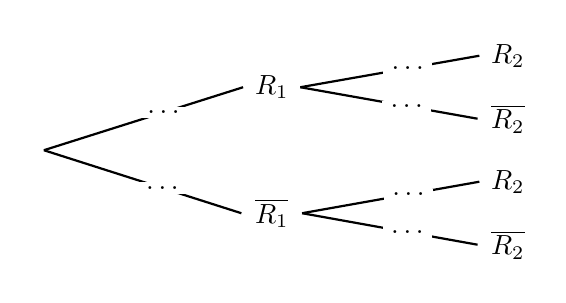
\begin{tikzpicture}[xscale=1,yscale=1,baseline={(R.base)}]
		
		\tikzstyle{fleche}=[-,>=latex,thick]
		\tikzstyle{noeud}=[fill=white,circle,inner sep=2pt]
		\tikzstyle{feuille}=[fill=white,circle,inner sep=2pt]
		\tikzstyle{etiquette}=[pos=0.6,fill=white, inner xsep=3pt, inner ysep=1.5pt]
		
		\def\DistanceInterNiveaux{3}
		\def\DistanceInterFeuilles{0.8}
		
		\def\NiveauA{(0)*\DistanceInterNiveaux}
		\def\NiveauB{(1)*\DistanceInterNiveaux}
		\def\NiveauC{(2)*\DistanceInterNiveaux}
		\def\InterFeuilles{(-1)*\DistanceInterFeuilles}
		
		\node[noeud] (R) at ({\NiveauA},{(1.5)*\InterFeuilles}) {};
		\node[noeud] (Ra) at ({\NiveauB},{(0.5)*\InterFeuilles}) {$R_1$};
		\node[feuille] (Raa) at ({\NiveauC},{(0)*\InterFeuilles}) {$R_2$};
		\node[feuille] (Rab) at ({\NiveauC},{(1)*\InterFeuilles}) {$\overline{R_2}$};
		\node[noeud] (Rb) at ({\NiveauB},{(2.5)*\InterFeuilles}) {$\overline{R_1}$};
		\node[feuille] (Rba) at ({\NiveauC},{(2)*\InterFeuilles}) {$R_2$};
		\node[feuille] (Rbb) at ({\NiveauC},{(3)*\InterFeuilles}) {$\overline{R_2}$};
		
		\draw[fleche] (R.east)--(Ra.west) node[etiquette] {$\dots$};
		\draw[fleche] (Ra.east)--(Raa.west) node[etiquette] {$\dots$};
		\draw[fleche] (Ra.east)--(Rab.west) node[etiquette] {$\dots$};
		\draw[fleche] (R.east)--(Rb.west) node[etiquette] {$\dots$};
		\draw[fleche] (Rb.east)--(Rba.west) node[etiquette] {$\dots$};
		\draw[fleche] (Rb.east)--(Rbb.west) node[etiquette] {$\dots$};
	\end{tikzpicture}
	\end{center}



















	\item On note $X$ la variable aléatoire donnant le gain algébrique du joueur, c'est-à-dire la différence entre la somme reçue après les deux tirages et les frais de participation au jeu de 1 euro.
	\begin{enumerate}
		\item Donner les valeurs prises par la variable aléatoire $X$.

		\item Montrer que $P(X=-1)=\dfrac{18}{100}$.

		\item Recopier sur votre feuille et compléter le tableau suivant donnant la loi de probabilité de $X$ :

		\begin{center}
		\begin{tblr}{colspec={X[2cm,c]XXX},hlines,vlines,width=0.7\linewidth}
			$k$ &  &  &  \\
			$P(X=k)$ &  &  &  \\
		\end{tblr}
		\end{center}

		\item Calculer l'espérance de $X$. Interpréter le résultat.
	\end{enumerate}
\end{enumerate}

\subsection*{Partie B}

	Dans cette partie, on considère que cette urne contient maintenant $n$ boules rouges et $10-n$ boules vertes où $n$ est un nombre entier naturel avec $0 \leq n \leq 10$.

	On note $Y$ la variable aléatoire donnant le gain algébrique après les deux tirages.

\begin{enumerate}
	\item Démontrer que \quad $E(Y)=\dfrac{4 n^{2}-20 n}{100}$.

	On expliquera la démarche mise en œuvre. Toute démarche, même incomplète, sera prise en compte dans la notation.

	\item Pour combien de boules rouges dans l'urne le jeu est-il équitable entre le joueur et le forain?
\end{enumerate}
